% Informe automático generado por asistente
\documentclass[11pt,a4paper]{article}
\usepackage[utf8]{inputenc}
\usepackage[T1]{fontenc}
\usepackage[spanish]{babel}
\usepackage{graphicx}
\usepackage{caption}
\usepackage{subcaption}
\usepackage{booktabs}
\usepackage{hyperref}
\usepackage{amsmath}
\usepackage{siunitx}
\usepackage{geometry}
\usepackage{float}
\geometry{margin=1in}
\hypersetup{colorlinks=true,linkcolor=blue,urlcolor=blue}

\title{Proyecto de Simulaci\'on: cobard\'ia vs altruismo}
\author{David S\'anchez Iglesias}
\date{mayo de 2026}

\begin{document}

\begin{titlepage}
  \centering
  \vspace*{1.5cm}

  {\Large \textbf{Universidad de La Habana}\\[0.3em]
   \large Facultad de Matemática y Computación}

  \vspace{2cm}
  \rule{\linewidth}{0.5pt}\\[0.4cm]
  {\LARGE \textbf{Proyecto de Simulaci\'on}}\\[0.3cm]
  {\large \textit{Cobard\'ia vs altruismo}}\\[0.2cm]
  \rule{\linewidth}{0.5pt}

  \vspace{1.5cm}

  \begin{tabular}{ll}
    \textbf{Estudiante:}  & {David S\'anchez Iglesias} \\[0.4em]
    \textbf{Grupo:}       & {C411} \\[0.4em]
    \textbf{Asignatura:}  & Simulación \\[0.4em]
    \textbf{Año académico:} & 4.º año, Curso 2025--2026 \\
  \end{tabular}

  \vspace{2cm}

  \textbf{Repositorio GitHub:}\\[0.3em]
  \url{https://github.com/Davidbestion/Simulation_cowardice_vs_altruism}

  \vfill
  {\small La Habana, mayo de 2026}
\end{titlepage}

\newpage

\tableofcontents
\newpage

\section{Introducci\'on}

Este trabajo estudia, mediante simulaci\'on computacional basada en agentes, la competencia evolutiva
entre estrategias de cooperaci\'on y de conducta ego\'ista en un entorno con depredaci\'on y recursos limitados.
El problema central es cl\'asico en biolog\'ia evolutiva: bajo qu\'e condiciones el altruismo puede mantenerse
cuando comparte poblaci\'on con individuos que se benefician sin asumir costes.

El proyecto modela poblaciones de criaturas cuyo comportamiento emerge de su genoma, compuesto por genes
que determinan tanto rasgos observables (por ejemplo, la se\~nal de barba verde) como reglas de acci\'on
ante depredadores. Sobre esa base se comparan estrategias de cobard\'ia, altruismo puro y altruismo selectivo,
analizando su efecto sobre la supervivencia, la reproducci\'on y la frecuencia g\'enica a lo largo del tiempo.

El objetivo del informe es doble: (i) describir con precisi\'on el modelo implementado y el dise\~no experimental,
y (ii) discutir qu\'e patrones son robustos y cu\'ales dependen de la estocasticidad de ejecuciones individuales.
De este modo, el estudio conecta la implementaci\'on del simulador con la interpretaci\'on evolutiva de los resultados.

\section{Modelo}

\subsection{Entidades y estado del sistema}

El sistema est\'a formado por una poblaci\'on de criaturas y un entorno discreto de \'arboles. Cada criatura posee
un \textit{genoma} (lista de genes) del que se derivan sus rasgos f\'isicos y su comportamiento frente al depredador.
En la implementaci\'on actual, el rasgo f\'isico relevante es \texttt{green\_beard}, utilizado por estrategias de
cooperaci\'on selectiva para decidir a qui\'en beneficiar.

El entorno contiene \texttt{num\_trees} \'arboles, cada uno con capacidad m\'axima de 2 criaturas por generaci\'on.
La presencia de un depredador en cada \'arbol se modela como una variable Bernoulli independiente con probabilidad
\texttt{predator\_probability}. Por tanto, en cada generaci\'on la mortalidad resulta de dos mecanismos:
\textit{hambre} (exceso de poblaci\'on respecto a la capacidad total) y \textit{depredaci\'on}.

\subsection{Din\'amica por generaci\'on}

La simulaci\'on opera en generaciones no solapadas. En cada generaci\'on se ejecutan, en orden, las siguientes fases:

\begin{enumerate}
    \item \textbf{Asignaci\'on a \'arboles:} las criaturas se distribuyen aleatoriamente en slots de alimentaci\'on
    (capacidad total igual a $2 \times \texttt{num\_trees}$). Si la poblaci\'on excede la capacidad, el excedente
    muere por hambre.
    \item \textbf{Encuentro con depredador:} en cada \'arbol ocupado se determina si hay depredador.
    Si no lo hay, todos sobreviven. Si lo hay y solo hay un ocupante, ese individuo muere.
    Si hay dos ocupantes, uno act\'ua como detector y la resoluci\'on depende del comportamiento definido por sus genes.
    \item \textbf{Reproducci\'on:} los supervivientes generan entre \texttt{offspring\_min} y
    \texttt{offspring\_max} descendientes; los progenitores no pasan a la siguiente generaci\'on.
    \item \textbf{Actualizaci\'on:} la nueva poblaci\'on queda formada por los descendientes y se registran
    las m\'etricas de la generaci\'on (tama\~no poblacional, muertes por hambre, muertes por depredaci\'on y frecuencias g\'enicas).
\end{enumerate}

\subsection{Estrategias g\'enicas consideradas}

Las criaturas dise\~nadas para este proyecto pueden portar genes que definen su comportamiento ante la presencia de un depredador en el \'arbol que ocupan.
Dichos genes pueden implementar distintas estrategias, que se resumen a continuaci\'on:

\begin{itemize}
    \item \texttt{CowardGene}: el detector huye y los dem\'as ocupantes del \'arbol no sobreviven.
    \item \texttt{AltruistGene}: el detector avisa a todos los dem\'as; su propia supervivencia ocurre con probabilidad
    \texttt{altruist\_escape\_prob}.
    \item \texttt{SelectiveAltruistGene}: el detector solo beneficia a individuos con \texttt{green\_beard}.
    \item \texttt{GreenBeardGene}: aporta la se\~nal f\'isica \texttt{green\_beard} sin comportamiento altruista asociado.
    \item \texttt{GreenBeardAltruistGene}: combina se\~nal \texttt{green\_beard} y altruismo selectivo.
\end{itemize}

Cuando una criatura posee m\'ultiples genes con comportamiento frente a depredador, se aplica una regla de prioridad
(campo \texttt{PRIORITY}) y ejecuta el gen de mayor prioridad que produzca una resoluci\'on v\'alida.

\subsection{Supuestos y alcance}

El modelo asume herencia directa del genoma, sin mutaci\'on, con apareamiento impl\'icito y generaciones discretas.
Asimismo, la asignaci\'on a \'arboles y la presencia de depredador se tratan como procesos aleatorios independientes
entre generaciones. Bajo estos supuestos, el simulador no pretende reproducir una especie concreta, sino ofrecer
un entorno controlado para estudiar estabilidad o colapso de estrategias cooperativas en funci\'on del coste individual,
la composici\'on inicial y la estructura de se\~nales de reconocimiento.

\section{Implementaci\'on}
\subsection{Estructura general del c\'odigo}

El c\'odigo principal de la simulaci\'on se encuentra en \texttt{src/simulation/core} y est\'a organizado por responsabilidad:

\begin{itemize}
	\item \texttt{simulation.py}: definiciones de configuraci\'on (\texttt{SimulationConfig}), la interfaz \texttt{Experiment} y el registro por generaci\'on (\texttt{GenerationReport}).
	\item \texttt{world.py}: definici\'on de \texttt{Tree} y \texttt{World} (capacidad de alimentaci\'on por \'arbol).
	\item \texttt{creature.py}: clase \texttt{Creature} que encapsula el genoma, rasgos f\'isicos y de comportamiento y la interfaz para responder ante un depredador.
	\item \texttt{genes.py}: implementaciones de los genes (p. ej. \texttt{CowardGene}, \texttt{AltruistGene}, \texttt{SelectiveAltruistGene}, \texttt{GreenBeardGene}, \texttt{GreenBeardAltruistGene}) y la API que deben seguir.
	\item \texttt{simulator.py}: la l\'ogica del ciclo diurno / por generaci\'on y la recogida de \texttt{GenerationReport}.
\end{itemize}

En adici\'on, la carpeta \texttt{src/simulation/instances} contiene los experimentos y sus generadores de genomas, y \texttt{src/simulation/analysis} las funciones de visualizaci\'on.

\subsection{Mundo y \'arboles}

El entorno se modela con la clase \texttt{Tree} (archivo \texttt{world.py}). Cada \texttt{Tree} tiene:
\begin{itemize}
	\item \texttt{tree\_id}: identificador int.
	\item \texttt{max\_capacity}: n\'umero m\'aximo de criaturas que pueden alimentarse (por defecto 2).
	\item \texttt{has\_predator}: bandera booleana que indica si en ese d\'ia hubo un depredador.
\end{itemize}

La clase \texttt{World} agrupa la colecci\'on de \texttt{Tree} y proporciona utilidades como la capacidad total (\texttt{total\_tree\_capacity}). El \texttt{Simulator} crea una lista de \texttt{Tree} cada generaci\'on basada en \texttt{cfg.num\_trees}.

\subsection{Criaturas y genoma}

Cada criatura es una instancia de \texttt{Creature} (archivo \texttt{creature.py}) construida con un \texttt{genome}, que es una lista de instancias de \texttt{Gene}.

Al inicializarse, \texttt{Creature} calcula dos diccionarios derivados iterando sobre su genoma:
\begin{itemize}
	\item \texttt{physical\_traits}: resultado de llamar \texttt{gene.apply\_physical\_traits(creature)} para cada gen.
	\item \texttt{behavioral\_traits}: resultado de \texttt{gene.apply\_behavioral\_traits(creature)}.
\end{itemize}

Estos diccionarios permiten consultas r\'apidas con \texttt{has\_trait(trait)} y facilitan que genes distintos aporten rasgos (por ejemplo \texttt{green\_beard}).

Adicionalmente \texttt{Creature} expone \texttt{has\_gene(gene\_type)} para comprobar si en el genoma hay una instancia de cierta clase de gen.

\subsection{Genes y comportamientos}

El contrato de un gen est\'a definido por la clase abstracta \texttt{Gene} (archivo \texttt{genes.py}). Los puntos clave son:
\begin{itemize}
	\item \texttt{name}: nombre legible del gen (usado en contadores de frecuencia).
	\item \texttt{PRIORITY}: entero que indica prioridad cuando varios genes implementan \texttt{predator\_behavior}.
	\item \texttt{apply\_physical\_traits(creature)}: devuelve cambios de rasgos f\'isicos.
	\item \texttt{apply\_behavioral\_traits(creature)}: devuelve rasgos de comportamiento.
	\item \texttt{predator\_behavior(notifier, assigned, cfg)}: opcional; debe devolver \texttt{(survivors, eaten\_count)} o \texttt{None} si no aplica.
\end{itemize}

Implementaciones concretas relevantes:
\begin{itemize}
	\item \texttt{CowardGene} (\texttt{PRIORITY=10}): el notificante huye y los dem\'as mueren (salvando al notificante).
	\item \texttt{AltruistGene} (\texttt{PRIORITY=20}): al avisar, todos los dem\'as escapan; el notificante escapa con probabilidad \texttt{cfg.altruist\_escape\_prob}.
	\item \texttt{SelectiveAltruistGene} (\texttt{PRIORITY=25}): altruismo selectivo solo hacia criaturas con \texttt{green\_beard}.
	\item \texttt{GreenBeardGene} (\texttt{PRIORITY=5}): aporta el rasgo f\'isico \texttt{green\_beard}.
	\item \texttt{GreenBeardAltruistGene} (\texttt{PRIORITY=30}): combina \texttt{green\_beard} + comportamiento altruista (prioridad alta).
\end{itemize}

El dise\~no de \texttt{predator\_behavior} permite que si una criatura posee m\'ultiples genes que definen comportamiento ante depredador,
	\texttt{Creature.handle\_predator} ordene dichos genes por \texttt{PRIORITY} (descendente) y ejecute en ese orden hasta que uno devuelva una resoluci\'on.

\subsection{Ciclo de simulaci\'on (por generaci\'on)}

La clase \texttt{Simulator} (archivo \texttt{simulator.py}) implementa el ciclo principal en \texttt{run()}:
\begin{enumerate}
	\item (Opcional) inicializaci\'on del RNG con \texttt{cfg.seed} para reproducibilidad.
	\item Llamada a \texttt{\_initialize\_population()} que usa \texttt{experiment.population\_specs} para construir la poblaci\'on inicial (vease m\'as abajo).
	\item Bucle de generaciones \texttt{for gen in 1..cfg.num\_generations}:
		\begin{enumerate}
			\item Crear \texttt{Tree} objetos y el \texttt{World} para esta generaci\'on.
			\item Calcular \texttt{total\_capacity} sumando \texttt{tree.max\_capacity}.
			\item Asignar criaturas a slots de \texttt{Tree} (ver secci\'on siguiente). Si la poblaci\'on excede la capacidad, algunos mueren por hambre (\texttt{starved}).
			\item Para cada \texttt{Tree} con ocupantes:
				\begin{itemize}
					\item Determinar si hay depredador: \texttt{t.has\_predator = random.random() < cfg.predator\_probability}.
					\item Si no hay depredador, todos los asignados sobreviven.
					\item Si hay depredador:
						\begin{itemize}
							\item Si solo hay un ocupante, ese muere (\texttt{eaten += 1}).
							\item Si hay m\'as de uno, se elige aleatoriamente un \texttt{detector} entre los asignados y se llama \texttt{detector.handle\_predator(assigned, cfg)}. Esta funci\'on delega en los genes (priorizados) y devuelve la lista de \texttt{survivors} y \texttt{eaten\_count}.
						\end{itemize}
				\end{itemize}
			\item Los supervivientes se reproducen: por cada superviviente se llama \texttt{Creature.reproduce()} que genera N descendientes (\texttt{random.randint(cfg.offspring\_min, cfg.offspring\_max)}). Los progenitores no se mantienen (morir\'ian al final del d\'ia), por tanto la nueva poblaci\'on est\'a formada solo por los descendientes.
			\item Se computan las frecuencias genicas en la nueva poblaci\'on y se crea un \texttt{GenerationReport} con las m\'etricas de la generaci\'on.
			\item Si la poblaci\'on queda vac\'ia, el bucle termina anticipadamente.
		\end{enumerate}
\end{enumerate}

\subsection{Asignaci\'on de criaturas a \'arboles}

La asignaci\'on se realiza en dos modos seg\'un la relaci\'on entre la poblaci\'on y la capacidad total:
\begin{itemize}
	\item Si \texttt{population\_start > total\_capacity}: se consideran \texttt{starved = population\_start - total\_capacity}. Se baraja la poblaci\'on (\texttt{random.shuffle}) y se seleccionan los \texttt{total\_capacity} que est\'an permitidos para alimentarse; estos se distribuyen llenando cada \'arbol hasta su capacidad.
	\item Si \texttt{population\_start <= total\_capacity}: se construye una lista de \texttt{slots} repitiendo cada \texttt{tree\_id} \texttt{max\_capacity} veces y se elige aleatoriamente \texttt{population\_start} slots con \texttt{random.sample(slots, k=population\_start)}. Cada criatura se asigna a un slot elegido.
\end{itemize}

Esta estrategia asegura que la asignaci\'on sea aleatoria, pero que respete la capacidad por \'arbol y el caso en que la poblaci\'on exceda dicha capacidad (muerte por hambre).

\subsection{Depredadores y detecci\'on}

La presencia de un depredador en un \'arbol se decide por evento Bernoulli con probabilidad \texttt{cfg.predator\_probability} por \'arbol (se eval\'ua cada generaci\'on). Si hay depredador y hay m\'as de una criatura en el \'arbol, se
escoge un \texttt{detector} aleatorio y se delega en \texttt{detector.handle\_predator} la resoluci\'on del enfrentamiento.

\texttt{Creature.handle\_predator} implementa la l\'ogica de resoluci\'on por genes: agrupa los genes que implementan \texttt{predator\_behavior}, los ordena por \texttt{PRIORITY} en orden descendente y ejecuta cada uno hasta obtener una respuesta no nula. Si ning\'un gen define comportamiento, la implementaci\'on por defecto devuelve \texttt{([], len(assigned))} (todos muertos).

El formato devuelto por un gen es \texttt{(survivors, eaten\_count)} donde \texttt{survivors} es una lista de referencias a criaturas que escapan y \texttt{eaten\_count} indica cu\'antas son comidas por el depredador.

\subsection{Generaci\'on de genomas y experimento}

Cada \texttt{Experiment} define \texttt{population\_specs}, una lista de tuplas \texttt{(genome\_factory, fraction)} donde \texttt{genome\_factory()} debe devolver una lista de instancias de \texttt{Gene} (el genoma) y \texttt{fraction} indica la fracci\'on de la poblaci\'on inicial que tendr\'a ese genoma. \texttt{\_initialize\_population()} convierte esas fracciones en conteos enteros, corrige errores de redondeo y construye \texttt{Creature(genome=...)} para cada individuo.

Ejemplo: un experimento puede usar \texttt{lambda: [CowardGene()]} para crear individuos cuya lista \texttt{genome} contiene una sola instancia de \texttt{CowardGene}.

\subsection{Reproducci\'on y manejo del genoma}

La funci\'on \texttt{Creature.reproduce()} crea nuevos objetos \texttt{Creature} con el mismo campo \texttt{genome} que el progenitor. En la implementaci\'on actual, la lista del genoma se pasa tal cual a los descendientes; esto funciona si los genes son inmutables, pero se deber\'ia copiar el genoma si en el futuro se permitieran mutaciones a nivel de instancia.

\subsection{Inicializaci\'on, semilla y reproducibilidad}

La clase \texttt{SimulationConfig} define los par\'ametros controlables: \texttt{num\_trees}, \texttt{num\_generations}, \texttt{initial\_population}, \texttt{predator\_probability}, \texttt{offspring\_min}, \texttt{offspring\_max} y \texttt{seed} (entre otros). \texttt{Simulator.run()} llama a \texttt{random.seed(cfg.seed)} cuando \texttt{seed} no es \texttt{None}, lo que permite reproducir ejecuciones.

En la utilidad \texttt{run.py} se implementa la l\'ogica para repetir un experimento varias veces (\texttt{--repeats}) y para controlar si cada repetici\'on debe ser determinista (semillas \texttt{base + i}) o no (semillas \texttt{None} para variar con el RNG del sistema).

\subsection{Reportes}

Por cada generaci\'on \texttt{Simulator} construye un \texttt{GenerationReport} (definido en \texttt{simulation.py}) que contiene: \texttt{generation}, \texttt{population\_start}, \texttt{starved}, \texttt{eaten}, \texttt{survived}, \texttt{population\_end} y \texttt{gene\_frequencies} (mapa \texttt{nombre\_gene} -> fracci\'on relativa). Estos objetos se usan luego para generar las figuras y el an\'alisis agregado.

\subsection{Notas de extensibilidad y consideraciones de implementaci\'on}

\begin{itemize}
	\item La separaci\'on de responsabilidades facilita a\~nadir nuevos genes implementando \texttt{predator\_behavior} o \texttt{apply\_*\_traits}.
	\item Si se desea permitir la mutaci\'on de genomas es recomendable clonar la lista \texttt{genome} en \texttt{Creature.reproduce()} para evitar aliasing entre instancias.
	\item La asignaci\'on actual de depredadores es independiente por \'arbol y por d\'ia; puede extenderse para modelar depredadores locales con distribuciones no Bernoulli.
\end{itemize}

% Fin de la seccion Implementacion


\graphicspath{{figuras/}}

\section{Dise\~no Experimental}

El dise\~no experimental sigue una l\'ogica de complejidad creciente: se parte de un escenario homog\'eneo de referencia,
se introduce progresivamente la competencia entre estrategias, y se a\~naden mecanismos de reconocimiento y cooperaci\'on selectiva
para examinar bajo qu\'e condiciones el altruismo puede mantenerse evolutivamente.
Los par\'ametros comunes a todas las simulaciones se recogen en la Tabla~\ref{tab:params}.

\begin{table}[H]
\centering
\caption{Par\'ametros fijos del entorno de simulaci\'on.}
\label{tab:params}
\begin{tabular}{ll}
\toprule
Par\'ametro & Valor \\
\midrule
N\'umero de \'arboles                          & 25 \\
Poblaci\'on inicial                            & 80 individuos \\
Probabilidad de depredador por \'arbol        & 0{,}30 \\
Cr\'ias por superviviente por generaci\'on    & 1--2 \\
Semilla aleatoria (\texttt{seed})              & 42 \\
\bottomrule
\end{tabular}
\end{table}

\subsection{Estudio 1: l\'inea base de cobard\'ia pura}

\textbf{Objetivo.} Caracterizar la din\'amica poblacional y de supervivencia bajo una estrategia \'unica
para disponer de una referencia con la que comparar los estudios posteriores.

\textbf{Condiciones.} Se simula una poblaci\'on homog\'enea de individuos portadores de \texttt{CowardGene},
con 100 generaciones y $p_\text{escape}=0{,}50$ (configuraci\'on por defecto).
Se realiza una \'unica ejecuci\'on, suficiente para observar la din\'amica estacionaria.

\subsection{Estudio 2: viabilidad del altruismo puro frente a la cobard\'ia}

\textbf{Objetivo.} Determinar si el altruismo puro puede coexistir con o desplazar a la cobard\'ia,
y c\'omo var\'ia ese resultado al modificar la ventaja individual del altruista ($p_\text{escape}$).

\textbf{Condiciones.} La poblaci\'on inicial se divide al 50\,\% entre \texttt{CowardGene} y \texttt{AltruistGene}.
El individuo altruista avisa a todos los compa\~neros de \'arbol al detectar un depredador,
incurriendo en el riesgo de ser comido con probabilidad $1 - p_\text{escape}$.
Se contemplan dos valores del par\'ametro $p_\text{escape}$:

\begin{itemize}
    \item $p_\text{escape}=0{,}50$, durante 100 generaciones (1 ejecuci\'on exploratoria).
    \item $p_\text{escape}=0{,}90$, durante 200 generaciones.
    Para este segundo valor, se realizan primero una ejecuci\'on individual para observar la trayectoria concreta
    y a continuaci\'on 30 ejecuciones independientes para estimar la variabilidad entre runs
    y confirmar la robustez estad\'istica del resultado.
\end{itemize}

\subsection{Estudio 3: altruismo selectivo con se\~nal de reconocimiento}

\textbf{Objetivo.} Estudiar si el altruismo puro puede volverse evolutivamente estable cuando se lo dota de un mecanismo de
reconocimiento: la se\~nal f\'isica de barba verde (\textit{green beard}), que permite al individuo altruista cooperar
exclusivamente con otros portadores de esa misma se\~nal.
Una vez confirmada la viabilidad del mecanismo en la distribuci\'on por defecto (50\,\% de altruistas),
se examina c\'omo influyen dos factores en su estabilidad: la proporci\'on inicial de altruistas en la poblaci\'on y el coste
individual del altruismo ($p_\text{escape}$).

\textbf{Condiciones.} En todas las condiciones de este estudio el \texttt{GreenBeardAltruistGene} mantiene la se\~nal y el
comportamiento altruista completamente acoplados: todo individuo con barba verde es altruista selectivo y viceversa.
Se var\'ian dos factores de forma cruzada, dando lugar a seis condiciones simuladas con 30 ejecuciones cada una (200 generaciones):

\begin{enumerate}
    \item \textbf{Probabilidad de escape} ($p_\text{escape}$): 0{,}10 (coste alto del altruismo), 0{,}50 (coste moderado), 0{,}90 (coste bajo).
    \item \textbf{Proporci\'on inicial de altruistas selectivos}: 50\,\% de altruistas frente a 10\,\% de altruistas
    (con el 90\,\% o el 50\,\% restante compuesto por cobardes puros, respectivamente).
\end{enumerate}

Esta combinaci\'on $3 \times 2$ permite separar el efecto de $p_\text{escape}$ del efecto de la proporci\'on inicial
sobre la din\'amica de fijaci\'on o extinci\'on del gen altruista.

\subsection{Estudio 4: competencia con se\~nal y comportamiento desacoplados}

\textbf{Objetivo.} Examinar qu\'e sucede cuando la se\~nal de barba verde y la conducta altruista existen como genes independientes
que pueden segregarse por separado en la poblaci\'on.
En este escenario ninguna estrategia altruista tiene garant\'ia de que avisar a un portador de la se\~nal implique cooperaci\'on rec\'iproca.

\textbf{Condiciones.} La poblaci\'on inicial se distribuye equitativamente al 25\,\% entre cuatro fenotipos:
\texttt{CowardGene} (cobarde puro, sin se\~nal),
\texttt{GreenBeardGene}+\texttt{CowardGene} (porta la se\~nal pero act\'ua como cobarde),
\texttt{SelectiveAltruistGene} (altruismo selectivo hacia portadores de barba verde, sin poseer la se\~nal propia),
y \texttt{GreenBeardAltruistGene} (porta la se\~nal y el altruismo selectivo acoplados).
Se realizan 30 ejecuciones de 400 generaciones con $p_\text{escape}=0{,}50$,
extendiendo el horizonte temporal para observar posibles dinámicas de largo plazo.


\section{Resultados}

\subsection{Prueba 1: din\'amica de la cobard\'ia pura}

La poblaci\'on hom\'og\'enea de cobardes (\texttt{Experiment1}, \texttt{default\_config}, 1 ejecuci\'on) muestra una din\'amica estable a lo largo de las 100 generaciones simuladas (Figura~\ref{fig:p1-pop}).
El tama\~no poblacional al final de cada generaci\'on oscila entre aproximadamente 52 y 80 individuos,
reflejando el equilibrio din\'amico entre reproducci\'on y mortalidad por depredaci\'on y por hambre.
Este resultado establece la l\'inea base: bajo cobard\'ia pura la especie ni se extingue ni crece ilimitadamente,
y la frecuencia del gen cobarde se mantiene en el 100\,\% durante toda la simulaci\'on.

\begin{figure}[H]
    \centering
    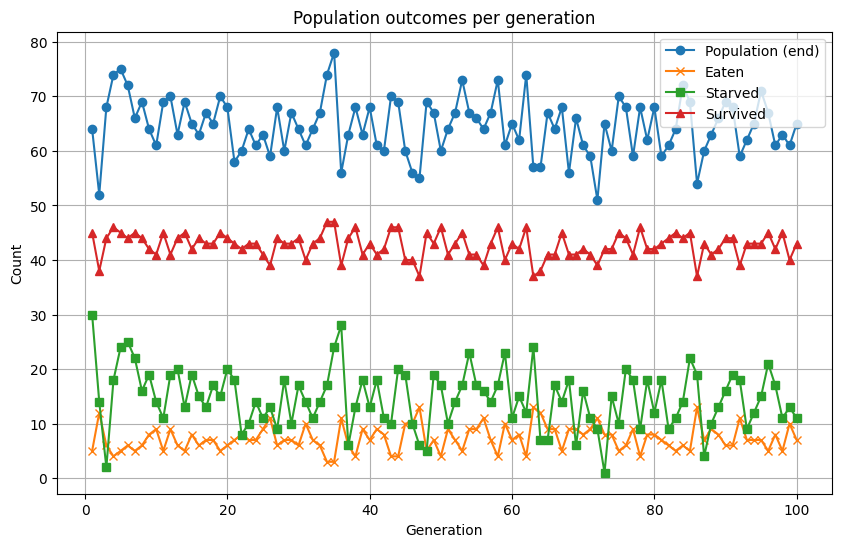
\includegraphics[width=0.80\textwidth]{fig01_exp1_population.png}
    \caption{Prueba~1 (\texttt{Experiment1}, \texttt{default\_config}): din\'amica poblacional durante 100 generaciones con cobard\'ia pura.}
    \label{fig:p1-pop}
\end{figure}

\subsection{Prueba 2: cobard\'ia frente a altruismo puro ($p_\text{escape}=0{,}50$)}

Introduciendo un 50\,\% de altruistas puros (\texttt{AltruistGene}) con la configuraci\'on por defecto (\texttt{default\_config}),
el gen altruista desaparece de la poblaci\'on con rapidez (Figura~\ref{fig:p2}).
La frecuencia del gen altruista cae desde el $\approx$50\,\% inicial hasta pr\'acticamente cero en torno a la generaci\'on 50,
tras lo cual la poblaci\'on queda compuesta exclusivamente por cobardes y su din\'amica reproduce la de la Prueba~1.
El altruista puro avisa a todos los individuos del \'arbol, incluyendo cobardes, que se benefician del aviso sin asumir ning\'un coste,
lo que confiere a los cobardes una aptitud relativa superior.

\begin{figure}[H]
    \centering
    \begin{subfigure}[b]{0.49\textwidth}
        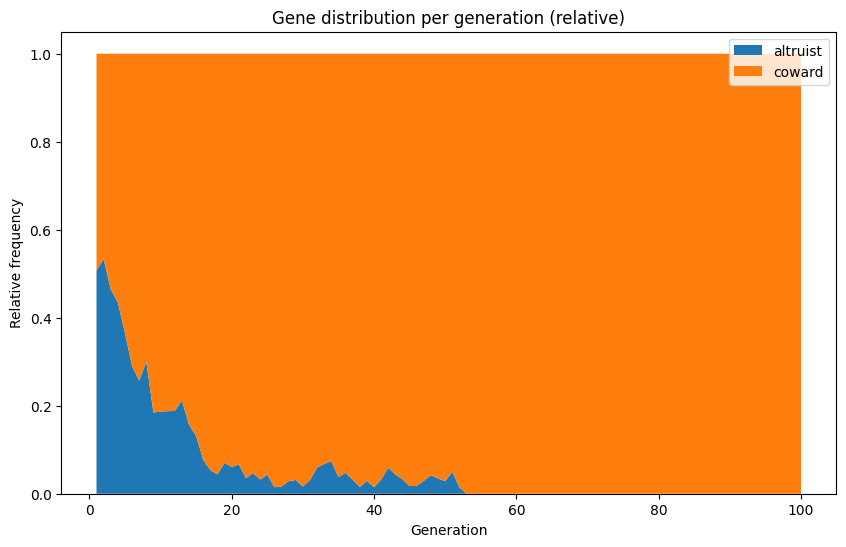
\includegraphics[width=\textwidth]{fig02_exp2_genes_run1.png}
        \caption{Distribuci\'on gen\'etica por generaci\'on.}
        \label{fig:p2-genes}
    \end{subfigure}
    \hfill
    \begin{subfigure}[b]{0.49\textwidth}
        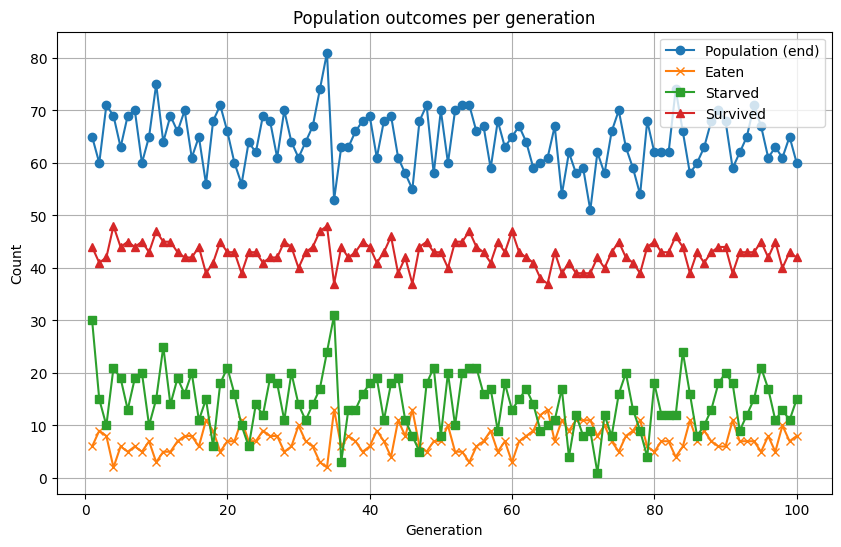
\includegraphics[width=\textwidth]{fig03_exp2_pop_run1.png}
        \caption{Din\'amica poblacional.}
        \label{fig:p2-pop}
    \end{subfigure}
    \caption{Prueba~2 (\texttt{Experiment2}, \texttt{default\_config}, 1 ejecuci\'on, $p_\text{escape}=0{,}50$).}
    \label{fig:p2}
\end{figure}

\subsection{Prueba 3: altruismo puro con alta probabilidad de escape ($p_\text{escape}=0{,}90$)}

Aumentar $p_\text{escape}$ al 90\,\% (\texttt{high\_escape\_prob}) produce un resultado llamativo en esta ejecuci\'{o}n
individual (Figura~\ref{fig:p3}): lejos de seguir el patr\'{o}n de la Prueba~2, la frecuencia del
altruista oscila err\'{a}ticamente durante las primeras $\sim$70 generaciones, alternando entre dominio
de cobardes y repuntes del altruista, lo que sugiere inestabilidad din\'{a}mica.A partir de la
generaci\'{o}n~70 el altruista comienza a imponerse de forma sostenida y alrededor de la
generaci\'{o}n~110 los cobardes se extinguen; el altruista termina fij\'{a}ndose en el 100\,\% de la
poblaci\'{o}n. Este resultado contrasta radicalmente con la Prueba~2 y plantea la pregunta de si,
con $p_\text{escape}$ suficientemente alto, el altruismo puro puede imponerse de forma general,
o si la victoria del altruista en esta ejecuci\'{o}n es un mero efecto del azar.

\begin{figure}[H]
    \centering
    \begin{subfigure}[b]{0.49\textwidth}
        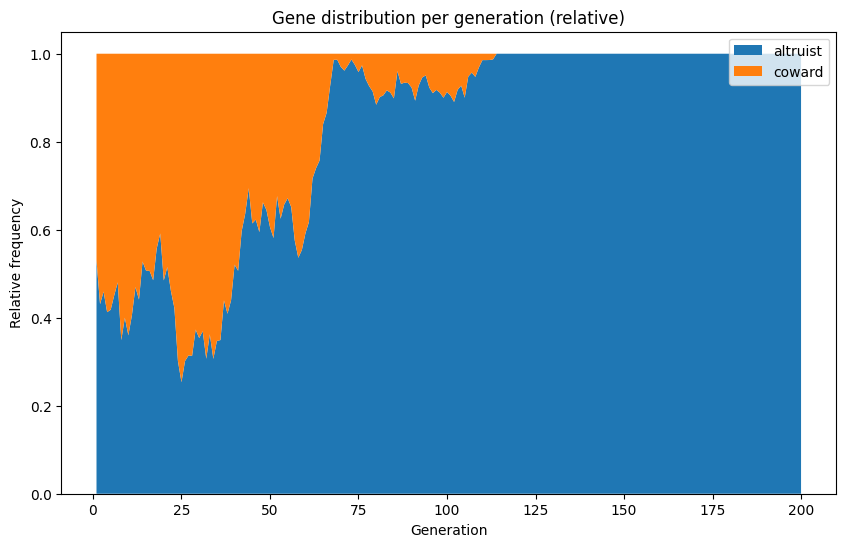
\includegraphics[width=\textwidth]{fig04_exp3_genes_run1.png}
        \caption{Distribuci\'on gen\'etica por generaci\'on.}
        \label{fig:p3-genes}
    \end{subfigure}
    \hfill
    \begin{subfigure}[b]{0.49\textwidth}
        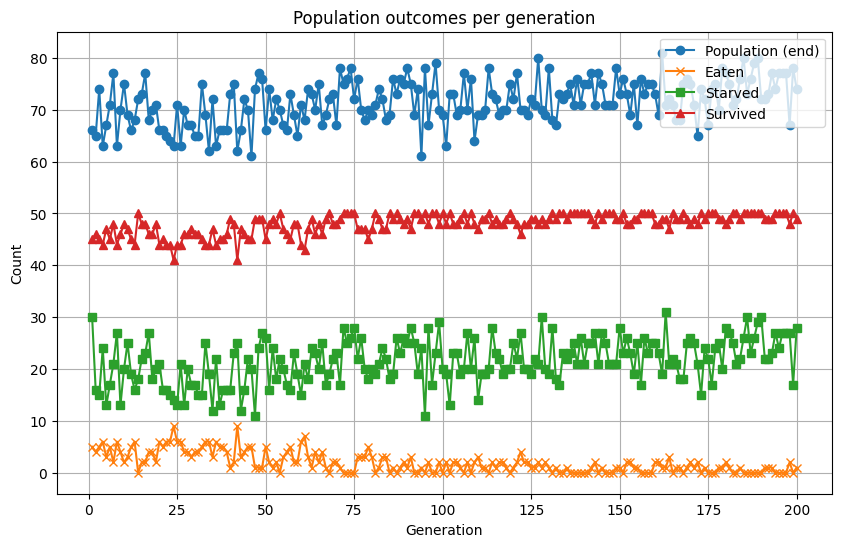
\includegraphics[width=\textwidth]{fig05_exp3_pop_run1.png}
        \caption{Din\'amica poblacional.}
        \label{fig:p3-pop}
    \end{subfigure}
    \caption{Prueba~3 (\texttt{Experiment2}, \texttt{high\_escape\_prob}, 1 ejecuci\'on, $p_\text{escape}=0{,}90$).}
    \label{fig:p3}
\end{figure}

\subsection{Prueba 4: verificaci\'on estad\'istica con 30 repeticiones ($p_\text{escape}=0{,}90$)}

Para determinar si la victoria del altruista observada en la Prueba~3 constituye el comportamiento
general o es un resultado puntual debido al azar, se replic\'{o} la misma condici\'{o}n exacta 30 veces.
La Figura~\ref{fig:p4} muestra la evoluci\'{o}n gen\'{e}tica agregada (media de los 30 runs).
El gen altruista decrece de forma sostenida desde el 50\,\% inicial hasta situarse en torno al
15--20\,\% al cabo de apenas 100 generaciones, sin que la media de los 30 runs muestre ning\'un repunte
ni tendencia hacia la fijaci\'on. La victoria del altruista observada en la Prueba~3 es por tanto
un resultado excepcional producto de la estocasticidad del modelo, no el comportamiento general:
promediando las trayectorias, el altruismo puro est\'a destinado a desaparecer incluso con
$p_\text{escape}=0{,}90$.
El tama\~no de la poblaci\'on (Figura~\ref{fig:p4-pop}) permanece estable y equivalente al de la Prueba~1.

\begin{figure}[H]
    \centering
    \begin{subfigure}[b]{0.49\textwidth}
        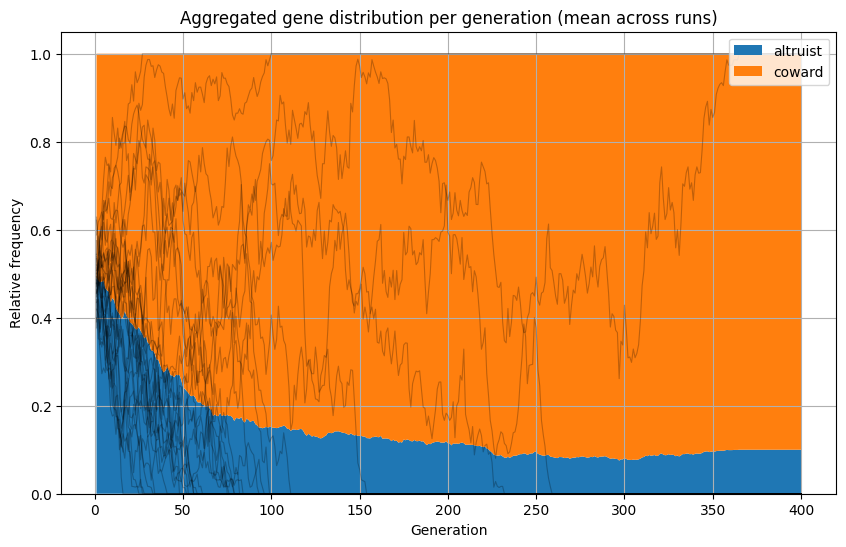
\includegraphics[width=\textwidth]{fig06_exp4_genes_agg.png}
        \caption{Evoluci\'on gen\'etica agregada (30 runs).}
        \label{fig:p4-genes}
    \end{subfigure}
    \hfill
    \begin{subfigure}[b]{0.49\textwidth}
        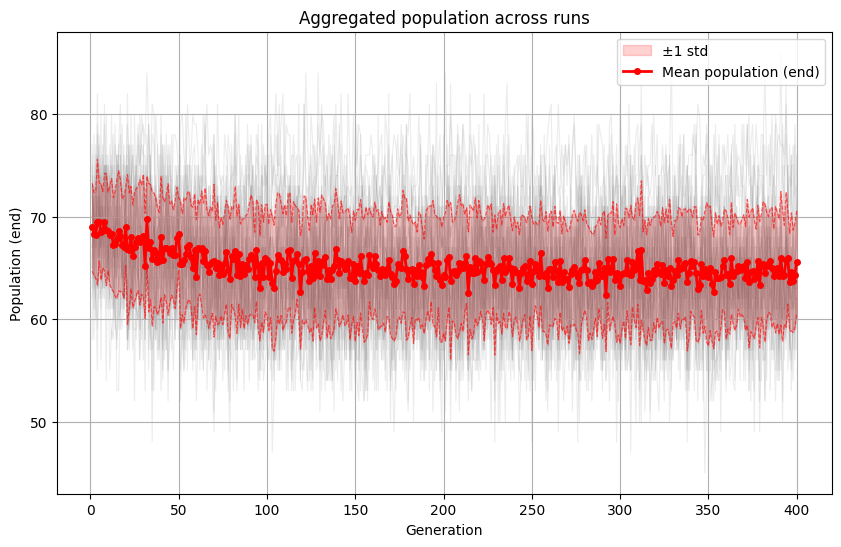
\includegraphics[width=\textwidth]{fig07_exp4_pop_agg.png}
        \caption{Poblaci\'on agregada (30 runs).}
        \label{fig:p4-pop}
    \end{subfigure}
    \caption{Prueba~4 (\texttt{Experiment2}, \texttt{high\_escape\_prob}, 30 repeticiones, $p_\text{escape}=0{,}90$).}
    \label{fig:p4}
\end{figure}

\subsection{Prueba 5: altruismo selectivo con se\~nal de barba verde}

Esta prueba estudia la viabilidad del \texttt{GreenBeardAltruistGene} bajo seis condiciones, resultado de cruzar
tres valores de $p_\text{escape}$ (0{,}10 / 0{,}50 / 0{,}90) con dos proporciones iniciales de altruistas:
50\,\% (mayoritaria) y 10\,\% (minoritaria), siendo el resto de la poblaci\'on cobardes puros en ambos casos.
En todo momento la se\~nal de barba verde y el comportamiento altruista van acoplados: no existen individuos
cobardes con barba verde.

\subsubsection*{Proporci\'on inicial del 50\,\% de altruistas selectivos}

Con la mitad de la poblaci\'on inicial compuesta por altruistas selectivos, el \texttt{GreenBeardAltruistGene}
se fija en la poblaci\'on en pocas generaciones bajo las tres probabilidades de escape (Figura~\ref{fig:p5-nogb}).
A $p_\text{escape}=0{,}50$ la fijaci\'on resulta evidente, pr\'acticamente extinguiendo a los cobardes
en el transcurso de 100 d\'ias; a $p_\text{escape}=0{,}10$ la ventaja de los altruistas es mucho menor,
y los datos reflejan esto mostrando un crecimiento mucho m\'as lento del altruista, aunque sostenido; y
a $p_\text{escape}=0{,}90$ el altruista se impone con rapidez, extinguiendo a los cobardes en 100 generaciones.
El altruismo selectivo elimina el coste de cooperar
con cobardes al avisar \'unicamente a otros portadores de la se\~nal, generando una ventaja que supera a la
cobard\'ia con independencia del coste individual del altruismo.

\begin{figure}[H]
    \centering
    \begin{subfigure}[b]{0.32\textwidth}
        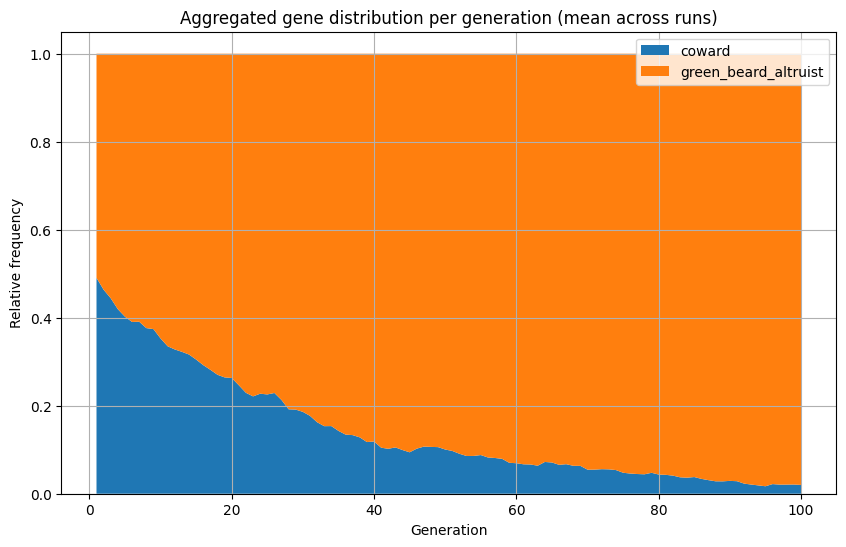
\includegraphics[width=\textwidth]{fig08_exp5_nogb_default.png}
        \caption{$p_\text{escape}=0{,}50$}
    \end{subfigure}
    \hfill
    \begin{subfigure}[b]{0.32\textwidth}
        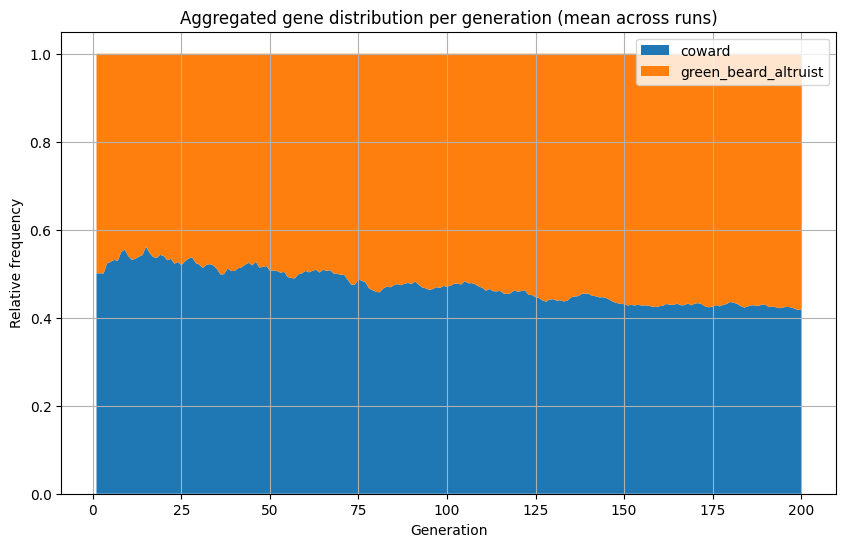
\includegraphics[width=\textwidth]{fig09_exp5_nogb_low.png}
        \caption{$p_\text{escape}=0{,}10$}
    \end{subfigure}
    \hfill
    \begin{subfigure}[b]{0.32\textwidth}
        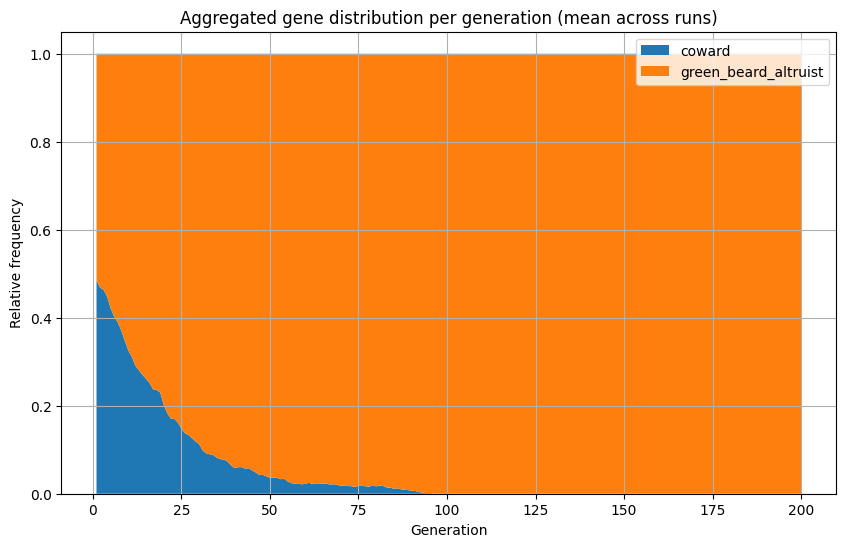
\includegraphics[width=\textwidth]{fig10_exp5_nogb_high.png}
        \caption{$p_\text{escape}=0{,}90$}
    \end{subfigure}
    \caption{Prueba~5, proporci\'on inicial del 50\,\% de altruistas selectivos (30 runs c/u).
    El gen \texttt{GreenBeardAltruistGene} se fija en la poblaci\'on en todos los casos.}
    \label{fig:p5-nogb}
\end{figure}

\subsubsection*{Proporci\'on inicial del 10\,\% de altruistas selectivos}

Reducir la presencia inicial del altruista al 10\,\% altera sustancialmente los resultados (Figura~\ref{fig:p5-gb}).
A $p_\text{escape}=0{,}10$ el gen cobarde domina completamente y el altruista selectivo aunque no desaparece en todas las ejecuciones,
s\'i se puede observar c\'omo la mayoria de las trayectorias se extinguen relativamente r\'apido, y las que persisten
muestran una evoluci\'on err\'atica con oscilaciones pronunciadas, sin tendencia clara hacia la fijaci\'on.
A $p_\text{escape}=0{,}50$ se observa c\'omo en la mayor\'ia de las ejecuciones se extingue el altruista si su poblaci\'on no crece
lo suficiente alrededor de los primeros 50 d\'ias, pero en las ejecuciones donde el altruista logra superar esa fase inicial de 
vulnerabilidad, se impone con rapidez superando a los cobardes y fij\'andose en la poblaci\'on.
A $p_\text{escape}=0{,}90$ se puede observar c\'omo en alrededor de la mitad de las ejecuciones se extingue el altruista en la 
fase inicial, pero en la otra mitad el altruista logra superar esa fase y se impone con rapidez, fij\'andose en la poblaci\'on.
Estos resultados muestran que la viabilidad del altruismo selectivo depende conjuntamente de la probabilidad que tienen
de escapar de los depredadores ($p_\text{escape}$) y de la proporci\'on inicial: a coste individual bajo, el
altruista puede prosperar incluso desde una posici\'on minoritaria; pero a coste alto, la masa cr\'itica inicial resulta determinante.

\begin{figure}[H]
    \centering
    \begin{subfigure}[b]{0.32\textwidth}
        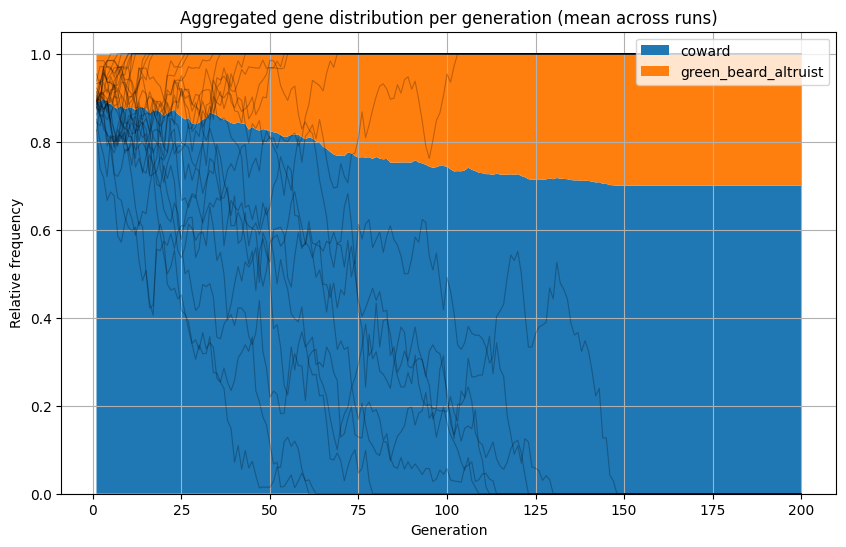
\includegraphics[width=\textwidth]{fig11_exp5_gb_default.png}
        \caption{$p_\text{escape}=0{,}50$}
    \end{subfigure}
    \hfill
    \begin{subfigure}[b]{0.32\textwidth}
        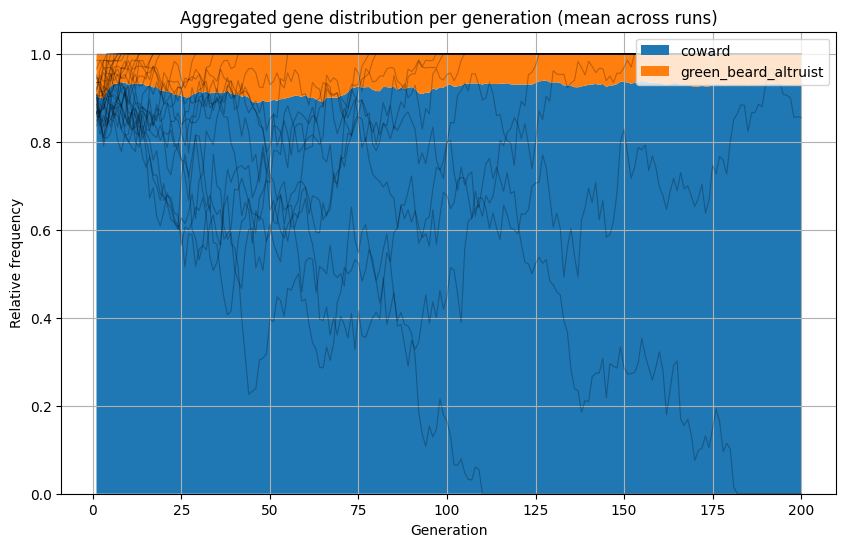
\includegraphics[width=\textwidth]{fig12_exp5_gb_low.png}
        \caption{$p_\text{escape}=0{,}10$}
    \end{subfigure}
    \hfill
    \begin{subfigure}[b]{0.32\textwidth}
        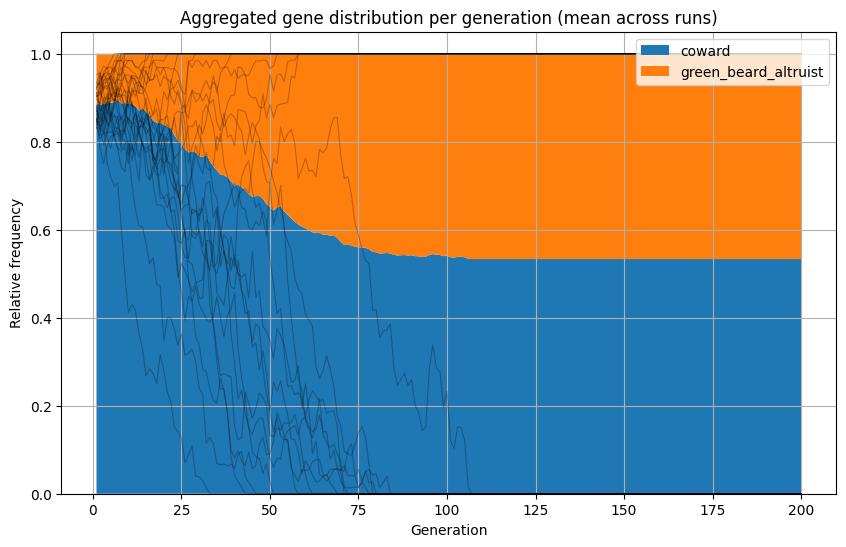
\includegraphics[width=\textwidth]{fig13_exp5_gb_high.png}
        \caption{$p_\text{escape}=0{,}90$}
    \end{subfigure}
    \caption{Prueba~5, proporci\'on inicial del 10\,\% de altruistas selectivos (30 runs c/u).
    La viabilidad del gen altruista depende del coste individual ($p_\text{escape}$).}
    \label{fig:p5-gb}
\end{figure}

\subsubsection*{Curiosidad: din\'amica de poblaci\'on con 10\,\% inicial de altruistas}

Como complemento descriptivo, la Figura~\ref{fig:p5-gb-pop} muestra la evoluci\'on del tama\~no
poblacional agregado (media y dispersi\'on entre runs) para el mismo bloque de comparaciones de la
Figura~\ref{fig:p5-gb}, es decir, manteniendo 10\,\% de altruistas selectivos iniciales y variando
\(p_\text{escape}\).
Se aprecia que con $p_\text{escape}=0{,}90$ la poblaci\'on media total presenta una tendencia ascendente
m\'as marcada a lo largo de las generaciones, mientras que en $p_\text{escape}=0{,}10$ y
$p_\text{escape}=0{,}50$ la evoluci\'on es m\'as plana y con menor incremento neto.
Esto se debe a que, al haber m\'as ejecuciones donde el altruista logra imponerse a los cobardes, 
el beneficio mutuo entre altruistas se traduce en una mayor supervivencia y reproducci\'on, 
lo que impulsa un crecimiento poblacional m\'as pronunciado. En contraste, con $p_\text{escape}=0{,}10$ 
la mayor parte de las ejecuciones terminan dominadas por cobardes, lo que limita el crecimiento poblacional 
y mantiene una din\'amica m\'as estable.

\begin{figure}[H]
    \centering
    \begin{subfigure}[b]{0.32\textwidth}
        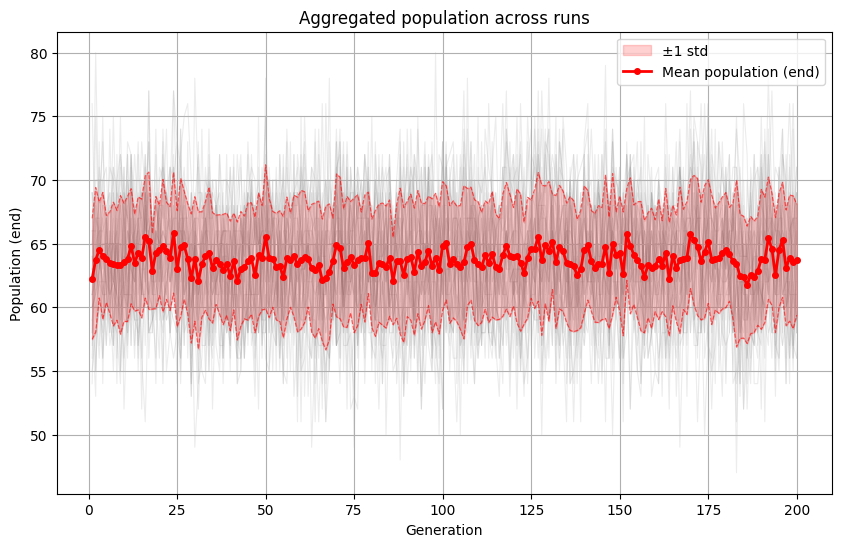
\includegraphics[width=\textwidth]{fig16_exp5_pop_low_10pct.png}
        \caption{$p_\text{escape}=0{,}10$}
    \end{subfigure}
    \hfill
    \begin{subfigure}[b]{0.32\textwidth}
        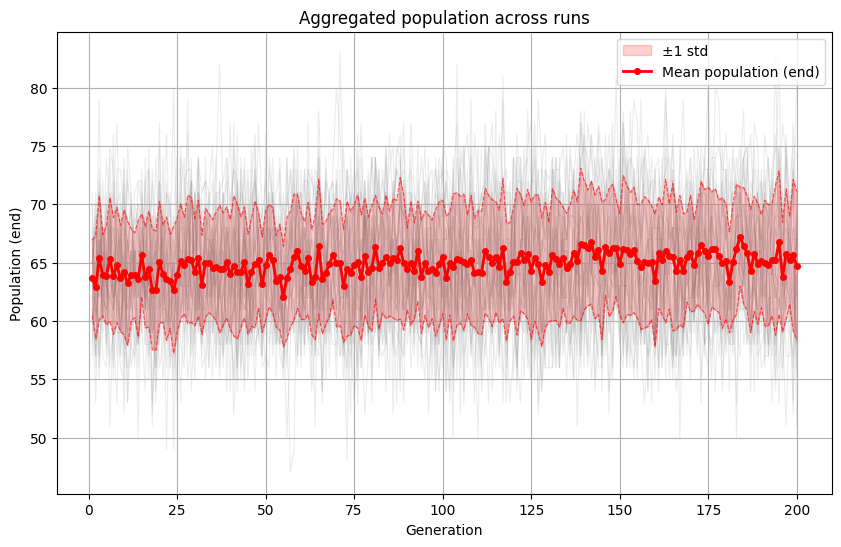
\includegraphics[width=\textwidth]{fig17_exp5_pop_default_10pct.png}
        \caption{$p_\text{escape}=0{,}50$}
    \end{subfigure}
    \hfill
    \begin{subfigure}[b]{0.32\textwidth}
        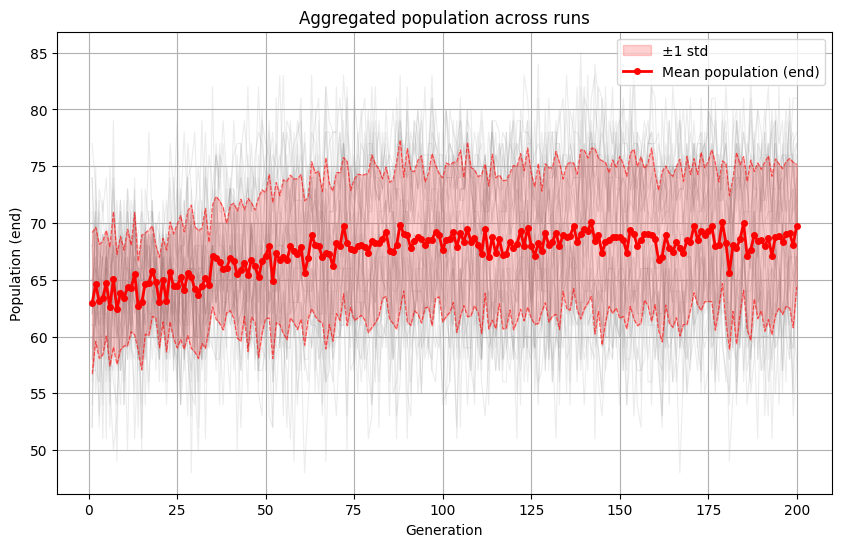
\includegraphics[width=\textwidth]{fig18_exp5_pop_high_10pct.png}
        \caption{$p_\text{escape}=0{,}90$}
    \end{subfigure}
    \caption{Din\'amica poblacional agregada en Prueba~5 con 10\,\% inicial de altruistas selectivos (30 runs c/u).
    A mayor $p_\text{escape}$ se observa un incremento m\'as claro de la poblaci\'on media final.}
    \label{fig:p5-gb-pop}
\end{figure}

\subsection{Prueba 6: separaci\'on de la se\~nal y del comportamiento altruista}

La Prueba~6 desacopla expl\'icitamente la se\~nal de barba verde del comportamiento altruista mediante \texttt{Experiment4},
donde \texttt{GreenBeardGene} y \texttt{SelectiveAltruistGene} coexisten como genes separados junto con \texttt{GreenBeardAltruistGene} y \texttt{CowardGene} (25\,\% cada uno, 400 generaciones).
La Figura~\ref{fig:p6} muestra que tanto \texttt{SelectiveAltruistGene} como \texttt{GreenBeardAltruistGene} desaparecen antes de la generaci\'on 50,
mientras que la poblaci\'on converge a un equilibrio entre cobarde puro ($\approx$55\,\%) y cobarde con barba verde ($\approx$45\,\%).
La barba verde pierde toda utilidad como se\~nal de reconocimiento al no garantizar el comportamiento cooperativo:
los altruistas que la usan como criterio de selecci\'on acaban cooperando con cobardes barbudos, pagando un coste sin obtener beneficio.
El tama\~no de la poblaci\'on (Figura~\ref{fig:p6-pop}) permanece estable en todos los casos, igual que en pruebas anteriores.

\begin{figure}[H]
    \centering
    \begin{subfigure}[b]{0.49\textwidth}
        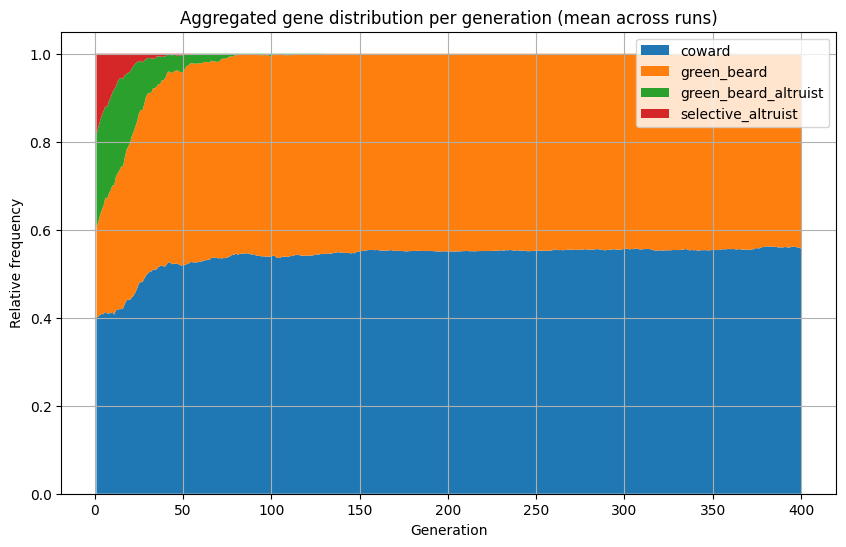
\includegraphics[width=\textwidth]{fig14_exp6_genes_agg.png}
        \caption{Evoluci\'on gen\'etica agregada (30 runs, 400 generaciones).}
        \label{fig:p6-genes}
    \end{subfigure}
    \hfill
    \begin{subfigure}[b]{0.49\textwidth}
        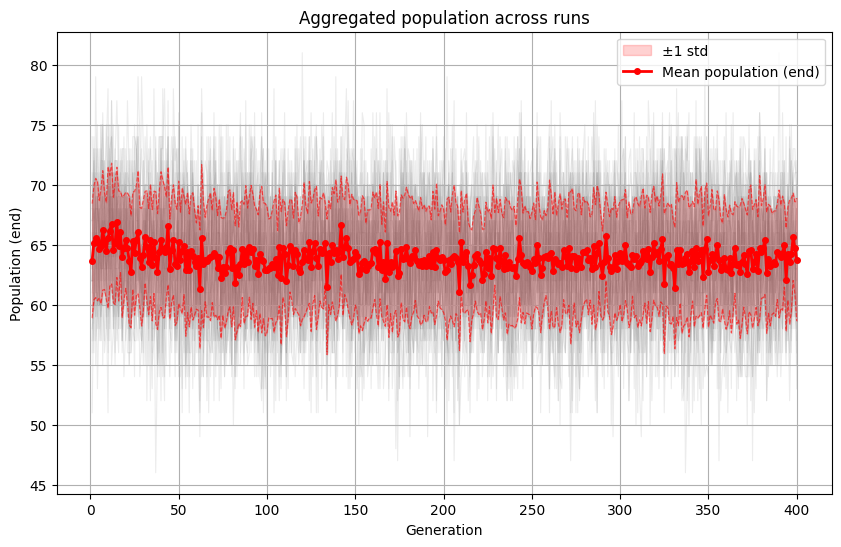
\includegraphics[width=\textwidth]{fig15_exp6_pop_agg.png}
        \caption{Poblaci\'on agregada (30 runs, 400 generaciones).}
        \label{fig:p6-pop}
    \end{subfigure}
    \caption{Prueba~6 (\texttt{Experiment4}, \texttt{default\_config}, 30 repeticiones).
    Las estrategias altruistas se extinguen antes de la generaci\'on 50.}
    \label{fig:p6}
\end{figure}

\section{Discusi\'on}

\subsection{Inestabilidad evolutiva del altruismo puro}

Las Pruebas~2, 3 y 4 demuestran que el altruismo puro (\texttt{AltruistGene}) es evolutivamente inestable cuando compite con la cobard\'ia,
con independencia de la probabilidad de escape del altruista.
El altruista puro avisa a todos los individuos de su \'arbol, incluyendo cobardes, que obtienen el beneficio del aviso sin asumir ning\'un coste.
Esto confiere a los cobardes una aptitud relativa superior y desplaza al altruista de la poblaci\'on,
en plena concordancia con la teor\'ia de la selecci\'on individual~\cite{hamilton1964}.
Aumentar $p_\text{escape}$ al 90\,\% (Prueba~3 y~4) solo ralentiza el proceso sin revertirlo.

\subsection{Efectividad del altruismo selectivo con se\~nal de barba verde}

Cuando la se\~nal de barba verde est\'a acoplada al comportamiento altruista y no existen explotadores de la se\~nal,
el altruismo selectivo es capaz de invadir y fijar una poblaci\'on mayoritariamente cobarde (Prueba~5, sin barba verde adicional).
Esto ocurre porque el \texttt{GreenBeardAltruistGene} dirige el coste del altruismo exclusivamente hacia otros portadores de la se\~nal,
que a su vez tambi\'en son altruistas; el beneficio mutuo genera una ventaja de aptitud sobre los cobardes.
Este resultado reproduce el mecanismo de la barba verde de Dawkins~\cite{dawkins1976} en un contexto computacional.

\subsection{Influencia de la proporci\'on inicial y del coste individual sobre el altruismo selectivo}

La Prueba~5 revela que la viabilidad del altruismo selectivo no s\'olo depende del mecanismo de reconocimiento,
sino de la interacci\'on entre la proporci\'on inicial de altruistas y el coste individual del comportamiento
($p_\text{escape}$).
Cuando los altruistas parten de una posici\'on mayoritaria (50\,\%), el gen se fija con independencia de
$p_\text{escape}$: la masa cr\'itica inicial es suficiente para que la cooperaci\'on selectiva genere
un beneficio neto superior a la cobard\'ia en cualquier escenario de coste.
Sin embargo, cuando parten de una minor\'ia (10\,\%), el resultado depende fuertemente de $p_\text{escape}$:
a coste alto (0{,}10) el altruista se extingue porque la escasez de portadores de la se\~nal hace que
cada encuentro altruista sea m\'as frecuentemente con un cobarde que con otro altruista,
mientras que a coste bajo (0{,}90) el altruista logra mantenerse en equilibrio estable.
Este resultado ilustra la importancia del efecto de masa cr\'itica en la evoluci\'on de la cooperaci\'on:
una estrategia cooperativa puede ser localmente estable por encima de cierto umbral de frecuencia
pero vulnerable a la extinci\'on si parte de una proporci\'on demasiado reducida~\cite{hamilton1964}.

La desactivaci\'on total del acoplamiento entre se\~nal y comportamiento (Prueba~6) produce el colapso
irreversible de ambas estrategias altruistas antes de la generaci\'on 50, confirmando que el mecanismo
de barba verde s\'olo es evolutivamente estable cuando la se\~nal implica de forma fiable el comportamiento
cooperativo~\cite{zahavi1975}.

\subsection{Robustez del tama\~no poblacional}

Una observaci\'on transversal a todas las pruebas es que la composici\'on gen\'etica determina la \textit{estructura} de la poblaci\'on (qu\'e estrategia domina) pero no su \textit{tama\~no}.
En todos los escenarios la poblaci\'on oscila en un rango similar al de la Prueba~1, determinado fundamentalmente por la capacidad del entorno (25 \'arboles) y la tasa reproductiva (1--2 cr\'ias por superviviente).

\section{Conclusiones}

\begin{enumerate}
    \item El altruismo puro no es evolutivamente estable en el modelo implementado:
    desaparece de la poblaci\'on independientemente de la probabilidad de escape del altruista (Pruebas 2--4).
    
    \item El altruismo selectivo mediado por la se\~nal de barba verde puede fijarse en la poblaci\'on cuando los altruistas parten de una proporci\'on inicial mayoritaria (50\,\%), con independencia del coste individual del altruismo (Prueba~5).
    
    \item Cuando los altruistas parten de una proporci\'on inicial reducida (10\,\%), la viabilidad del mecanismo depende del coste individual: a $p_\text{escape}$ baja, el gen altruista se extingue; a $p_\text{escape}$ alta, persiste en un equilibrio estable (Prueba~5). Esto sugiere la existencia de un umbral de masa cr\'itica por debajo del cual el altruismo selectivo no puede prosperar.
    
    \item Cuando la se\~nal y el comportamiento altruista se desacoplan como genes independientes, ambas estrategias altruistas (\texttt{GreenBeardAltruistGene} y \texttt{SelectiveAltruistGene}) se extinguen antes de la generaci\'on 50 y la poblaci\'on converge a cobardes puros o barbudos (Prueba 6).
    
    \item El tama\~no de la poblaci\'on es robusto frente a la composici\'on gen\'etica y queda determinado por los par\'ametros ecol\'ogicos del entorno.
\end{enumerate}

\medskip
Los resultados obtenidos sugieren que la evoluci\'on del altruismo requiere mecanismos de reconocimiento que sean dif\'iciles de falsificar
---como el parentesco gen\'etico real o la reciprocidad en interacciones repetidas---,
ninguno de los cuales ha sido modelado en el presente trabajo y constituye una l\'inea natural de extensi\'on futura.

\begin{thebibliography}{9}
\bibitem{hamilton1964}
    W.D. Hamilton, \textit{The genetical evolution of social behaviour I \& II},
    Journal of Theoretical Biology, 7(1):1--52, 1964.

\bibitem{dawkins1976}
    R. Dawkins, \textit{The Selfish Gene},
    Oxford University Press, Oxford, 1976.

\bibitem{zahavi1975}
    A. Zahavi, \textit{Mate selection---a selection for a handicap},
    Journal of Theoretical Biology, 53(1):205--214, 1975.
\end{thebibliography}

\end{document}

\subsubsection*{Variante A: $p_\text{escape}=0{,}50$}

Con una probabilidad de escape del altruista del 50\,\%, el gen altruista desaparece con rapidez de la poblaci\'on.
La Figura~\ref{fig:exp2-genes} muestra c\'omo la frecuencia del gen altruista cae de un valor inicial del 52\,\% hasta pr\'acticamente cero en torno a la generaci\'on 50, tras lo cual la poblaci\'on queda compuesta exclusivamente por cobardes.
La din\'amica poblacional (Figura~\ref{fig:exp2-pop}) es comparable a la del Experimento 1 tras la fijaci\'on del gen cobarde,
con supervivientes estables en torno a 40--45 individuos por generaci\'on.

\begin{figure}[H]
    \centering
    \begin{subfigure}[b]{0.49\textwidth}
        \includegraphics[width=\textwidth]{fig2_exp2_genes_run1.png}
        \caption{Distribuci\'on de genes por generaci\'on (1 ejecuci\'on, $p_\text{escape}=0{,}50$).}
        \label{fig:exp2-genes}
    \end{subfigure}
    \hfill
    \begin{subfigure}[b]{0.49\textwidth}
        \includegraphics[width=\textwidth]{fig3_exp2_population_run1.png}
        \caption{Din\'amica poblacional por generaci\'on (1 ejecuci\'on, $p_\text{escape}=0{,}50$).}
        \label{fig:exp2-pop}
    \end{subfigure}
    \caption{Experimento 2, Variante A: cobard\'ia frente a altruismo puro con $p_\text{escape}=0{,}50$.}
\end{figure}

\subsubsection*{Variante B: $p_\text{escape}=0{,}90$ (30 repeticiones, 200 generaciones)}

Incluso al aumentar la probabilidad de escape del altruista hasta el 90\,\%, el gen altruista no logra establecerse en la poblaci\'on.
Como muestra la Figura~\ref{fig:exp2-agg-genes}, la frecuencia media del gen altruista desciende de forma mon\'otona desde el 50\,\% inicial
hasta situarse en torno al 15\,\%--20\,\% al final de las 200 generaciones.
La variabilidad entre ejecuciones es considerable en las primeras generaciones pero se reduce progresivamente.
La din\'amica poblacional agregada (Figura~\ref{fig:exp2-agg-pop}) permanece estable con una media de la poblaci\'on final de
aproximadamente 65 individuos y una desviaci\'on est\'andar de $\pm$3--5, lo que indica que la composici\'on gen\'etica no afecta significativamente al tama\~no total de la poblaci\'on.

\begin{figure}[H]
    \centering
    \begin{subfigure}[b]{0.49\textwidth}
        \includegraphics[width=\textwidth]{fig4_exp2_genes_agg_high.png}
        \caption{Distribuci\'on gen\'etica agregada (30 runs, $p_\text{escape}=0{,}90$).}
        \label{fig:exp2-agg-genes}
    \end{subfigure}
    \hfill
    \begin{subfigure}[b]{0.49\textwidth}
        \includegraphics[width=\textwidth]{fig5_exp2_pop_agg_high.png}
        \caption{Poblaci\'on final agregada (30 runs, $p_\text{escape}=0{,}90$).}
        \label{fig:exp2-agg-pop}
    \end{subfigure}
    \caption{Experimento 2, Variante B: cobard\'ia frente a altruismo puro con $p_\text{escape}=0{,}90$, 30 repeticiones.}
\end{figure}

\subsection{Experimento 3: cobard\'ia frente a altruismo selectivo con se\~nal de parentesco}

\subsubsection*{Variante A: $p_\text{escape}=0{,}50$, sin barba verde en la poblaci\'on cobarde}

La introducci\'on de la se\~nal de barba verde como mecanismo de reconocimiento alter\'o dr\'asticamente la din\'amica evolutiva.
Partiendo de una frecuencia inicial del \texttt{GreenBeardAltruistGene} del 10\,\%, este gen se fija en la poblaci\'on en pocas generaciones.
La Figura~\ref{fig:exp3-default} muestra c\'omo en torno a la generaci\'on 5--10 el gen altruista con barba verde ya supera el 90\,\% de la poblaci\'on,
alcanzando la cuasi-fijaci\'on (frecuencia $>$95\,\%) antes de la generaci\'on 40.

\begin{figure}[H]
    \centering
    \includegraphics[width=0.75\textwidth]{fig6_exp3_genes_agg_default.png}
    \caption{Experimento 3, Variante A: distribuci\'on gen\'etica agregada (30 runs, $p_\text{escape}=0{,}50$).
    El gen \texttt{green\_beard\_altruist} alcanza la cuasi-fijaci\'on en pocas generaciones.}
    \label{fig:exp3-default}
\end{figure}

\subsubsection*{Variante B: $p_\text{escape}=0{,}10$, con 10\,\% de barba verde en la poblaci\'on cobarde}

Reducir la probabilidad de escape del altruista al 10\,\% e introducir barba verde en el 10\,\% inicial de los cobardes invierte completamente el resultado.
Como se aprecia en la Figura~\ref{fig:exp3-low}, el gen cobarde domina desde el inicio y se mantiene con una frecuencia superior al 90\,\% durante todo el experimento.
La presencia de individuos cobardes portadores de la se\~nal (barba verde sin altruismo) neutraliza el beneficio del reconocimiento,
ya que los altruistas que avisan a cobardes barbudos no reciben reciprocidad, pagando el coste del altruismo sin obtener beneficio.

\begin{figure}[H]
    \centering
    \includegraphics[width=0.75\textwidth]{fig7_exp3_genes_agg_low.png}
    \caption{Experimento 3, Variante B: distribuci\'on gen\'etica agregada (30 runs, $p_\text{escape}=0{,}10$,
    con 10\,\% de barba verde en cobardes). El gen cobarde domina durante todo el experimento.}
    \label{fig:exp3-low}
\end{figure}

\subsubsection*{Variante C: $p_\text{escape}=0{,}90$, con 10\,\% de barba verde en la poblaci\'on cobarde}

Con una probabilidad de escape del 90\,\% e individuos cobardes con barba verde, se observa un equilibrio intermedio.
La Figura~\ref{fig:exp3-high} muestra que el gen cobarde converge a una frecuencia estable en torno al 70\,\%,
mientras que el altruista con barba verde se mantiene en aproximadamente el 30\,\%.
En este escenario, el coste de avisar a cobardes barbudos queda parcialmente compensado por la alta probabilidad de escape del propio altruista,
lo que le permite persistir en la poblaci\'on como estrategia minoritaria.

\begin{figure}[H]
    \centering
    \includegraphics[width=0.75\textwidth]{fig8_exp3_genes_agg_high.png}
    \caption{Experimento 3, Variante C: distribuci\'on gen\'etica agregada (30 runs, $p_\text{escape}=0{,}90$,
    con 10\,\% de barba verde en cobardes). Convergencia a un equilibrio cobarde--altruista en torno a 70--30\,\%.}
    \label{fig:exp3-high}
\end{figure}

\subsection{Experimento 4: competici\'on de cuatro estrategias}

El experimento de cuatro fenotipos proporciona el escenario m\'as complejo y revela la vulnerabilidad de las estrategias altruistas ante la presencia de individuos que explotan la se\~nal sin cooperar.
La Figura~\ref{fig:exp4-genes} muestra que tanto el \texttt{SelectiveAltruistGene} como el \texttt{GreenBeardAltruistGene} desaparecen de la poblaci\'on antes de las primeras 50 generaciones,
mientras que el fenotipo \texttt{GreenBeard}+\texttt{Coward} y el cobarde puro dominan el resto de la simulaci\'on.
A partir de la generaci\'on 50, la poblaci\'on converge a un equilibrio entre el cobarde puro ($\approx$55\,\%) y el cobarde portador de barba verde ($\approx$45\,\%),
que se mantiene estable hasta la generaci\'on 400.

La din\'amica poblacional (Figura~\ref{fig:exp4-pop}) no muestra diferencias sustanciales respecto a los experimentos anteriores:
la poblaci\'on media al final de cada generaci\'on oscila entre 62 y 68 individuos con una desviaci\'on est\'andar de $\pm$4--5,
confirmando que la composici\'on gen\'etica incide sobre la estructura de la poblaci\'on pero no sobre su tama\~no global.

\begin{figure}[H]
    \centering
    \begin{subfigure}[b]{0.49\textwidth}
        \includegraphics[width=\textwidth]{fig9_exp4_genes_agg.png}
        \caption{Distribuci\'on gen\'etica agregada (30 runs, 400 generaciones).}
        \label{fig:exp4-genes}
    \end{subfigure}
    \hfill
    \begin{subfigure}[b]{0.49\textwidth}
        \includegraphics[width=\textwidth]{fig10_exp4_pop_agg.png}
        \caption{Poblaci\'on final agregada (30 runs, 400 generaciones).}
        \label{fig:exp4-pop}
    \end{subfigure}
    \caption{Experimento 4: competici\'on de cuatro estrategias, 30 repeticiones.
    Las estrategias altruistas desaparecen antes de la generaci\'on 50.}
\end{figure}

\section{Discusi\'on}

\subsection{Inestabilidad evolutiva del altruismo puro}

Los resultados del Experimento~2 reflejan el problema cl\'asico del altruismo en biolog\'ia evolutiva:
una estrategia altruista que beneficia a individuos no emparentados (sin mecanismo de reconocimiento) resulta evolutivamente inestable cuando compite con estrategias ego\'istas~\cite{hamilton1964}.
En el modelo implementado, el altruista puro avisa a todos los individuos de su \'arbol, incurriendo en un coste personal (probabilidad de ser comido)
para beneficiar tambi\'en a cobardes. Dado que los cobardes obtienen el beneficio de la alerta sin reciprocar, su aptitud relativa es mayor y se imponen.
La Prueba~3 muestra que una sola ejecuci\'{o}n con $p_\text{escape}=0{,}90$ puede, por efecto del azar,
dar lugar a la victoria completa del altruista; sin embargo, la Prueba~4 demuestra que este resultado
es excepcional: promediando 30 repeticiones, el gen altruista declina de forma sostenida y no se fija.
Este resultado es coherente con la predicci\'on de Hamilton~\cite{hamilton1964}: el altruismo no dirigido no puede mantenerse si la selecci\'on opera sobre individuos no emparentados.

\subsection{El efecto de la se\~nal de reconocimiento (barba verde)}

El mecanismo de barba verde (\textit{green beard}), introducido en el Experimento~3, demuestra ser altamente efectivo bajo ciertas condiciones.
Cuando la se\~nal est\'a acoplada funcionalmente al comportamiento altruista (solo los individuos altruistas portan la barba),
el gen \texttt{GreenBeardAltruistGene} es capaz de invadir y fijar una poblaci\'on mayoritariamente cobarde en pocas generaciones (Variante~A).
Esto ocurre porque el altruismo selectivo elimina el coste de cooperar con individuos que no reciprocan:
al avisar \'unicamente a otros portadores de barba verde, el altruista maximiza el beneficio del comportamiento cooperativo.

Sin embargo, la Variante~B del Experimento~3 pone de manifiesto la fragilidad de este mecanismo:
basta con que el 10\,\% inicial de la poblaci\'on cobarde porte tambi\'en la se\~nal para que el equilibrio se invierta completamente.
Los altruistas que avisan a cobardes barbudos asumen el riesgo de depredaci\'on sin obtener ning\'un beneficio de esos individuos,
lo que reduce dr\'asticamente su aptitud. Este fen\'omeno constituye un caso de explotaci\'on de la se\~nal o \textit{cheating}~\cite{dawkins1976},
y su efecto depende cr\'iticamente de $p_\text{escape}$: solo con una probabilidad muy alta (Variante~C, 90\,\%)
los altruistas logran coexistir con los cobardes barbudos, aunque no domin\'andolos.

\subsection{Colapso de las estrategias altruistas ante la diversidad de se\~nales}

El Experimento~4 extiende el an\'alisis al escenario de cuatro estrategias y confirma la predicci\'on del Experimento~3~(Variante~B).
La presencia de individuos \texttt{GreenBeard+Coward} (portadores de la se\~nal sin el comportamiento asociado) supone una presi\'on selectiva fatal para ambas estrategias altruistas:
el \texttt{GreenBeardAltruistGene} pierde rapidamente porque avisa a cobardes barbudos,
y el \texttt{SelectiveAltruistGene} desaparece porque avisa a cualquier portador de barba verde sin distinguir si tambi\'en son altruistas.
El resultado es la fijaci\'on de los cobardes como \'unica estrategia viable, con independencia de si portan o no la se\~nal de barba verde,
cuya funci\'on pierde todo valor de reconocimiento.

Este resultado ilustra el principio de que la estabilidad evolutiva de una se\~nal de parentesco requiere que la se\~nal sea fiel,
es decir, que su presencia implique de forma confiable el comportamiento cooperativo~\cite{zahavi1975}.
En cuanto la se\~nal puede desacoplarse del comportamiento (como ocurre con \texttt{GreenBeard+Coward}),
su valor informativo colapsa y el altruismo asociado deja de ser una estrategia viable.

\subsection{Estabilidad del tama\~no poblacional}

Una observaci\'on transversal a todos los experimentos es que la composici\'on gen\'etica afecta a la \textit{estructura} (qui\'enes sobreviven)
pero no al \textit{tama\~no} de la poblaci\'on.
En todos los escenarios la poblaci\'on media al final de cada generaci\'on se sit\'ua entre 62 y 70 individuos con baja varianza ($\pm$5),
lo que indica que el modelo alcanza r\'apidamente un equilibrio din\'amico determinado principalmente por la capacidad del entorno (25 \'arboles $\times$ 2 plazas = 50 plazas) y la tasa reproductiva (1--2 cr\'ias por superviviente).

\section{Conclusiones}

Las simulaciones realizadas permiten extraer las siguientes conclusiones:

\begin{enumerate}
    \item El altruismo puro (\texttt{AltruistGene}) no es una estrategia evolutivamente estable cuando compite con la cobard\'ia, independientemente de la probabilidad de escape del altruista.
    El gen altruista desaparece en todas las ejecuciones del Experimento~2, coincidiendo con la teor\'ia de la selecci\'on individual.
    
    \item La se\~nal de reconocimiento (barba verde) puede hacer viable el altruismo selectivo si la se\~nal es un indicador fiable del comportamiento cooperativo.
    En ausencia de explotadores de la se\~nal, el \texttt{GreenBeardAltruistGene} domina la poblaci\'on con rapidez.
    
    \item La presencia de individuos que portan la se\~nal sin el comportamiento asociado (\textit{cheaters}) destruye la efectividad del altruismo selectivo.
    Una frecuencia inicial del 10\,\% de cobardes barbudos es suficiente para impedir la fijaci\'on del gen altruista cuando $p_\text{escape}=0{,}10$, y para reducir su frecuencia de equilibrio al 30\,\% cuando $p_\text{escape}=0{,}90$.
    
    \item En el escenario de cuatro estrategias, los cobardes portadores de la se\~nal actúan como par\'asitos sociales que aceleran la extinci\'on de ambos tipos de altruistas.
    La poblaci\'on converge a un equilibrio entre cobarde puro y cobarde barbudo, ambos funcionalmente equivalentes.
    
    \item El tama\~no de la poblaci\'on es robusto frente a la composici\'on gen\'etica y queda determinado principalmente por los par\'ametros ecol\'ogicos (capacidad del entorno y tasa reproductiva).
\end{enumerate}

\medskip
Estos resultados apuntan a que la evoluci\'on del altruismo requiere mecanismos robustos de reconocimiento que sean dif\'iciles de falsificar,
como el parentesco gen\'etico real (selecci\'on de parentela) o la reciprocidad en interacciones repetidas,
ninguno de los cuales ha sido modelado en el presente trabajo y constituye una direcci\'on natural de extensi\'on futura.

\begin{thebibliography}{9}
\bibitem{hamilton1964}
    W.D. Hamilton, \textit{The genetical evolution of social behaviour I \& II},
    Journal of Theoretical Biology, 7(1):1--52, 1964.

\bibitem{dawkins1976}
    R. Dawkins, \textit{The Selfish Gene},
    Oxford University Press, Oxford, 1976.

\bibitem{zahavi1975}
    A. Zahavi, \textit{Mate selection---a selection for a handicap},
    Journal of Theoretical Biology, 53(1):205--214, 1975.
\end{thebibliography}

\end{document}

